\documentclass[10pt]{beamer}

% Theme and Styling
\usetheme{Madrid}
\usecolortheme{whale}
\setbeamertemplate{navigation symbols}{}
\setbeamertemplate{footline}[frame number]

% Packages
\usepackage[utf8]{inputenc}
\usepackage[T1]{fontenc}
\usepackage{lmodern}
\usepackage{graphicx}
\usepackage{tikz}
\usetikzlibrary{arrows.meta, positioning, shapes.geometric}
\usepackage{listings}
\usepackage{xcolor}

% Colors
\definecolor{medblue}{RGB}{0, 114, 187}
\definecolor{medgreen}{RGB}{46, 204, 113}
\setbeamercolor{title}{fg=white, bg=medblue}
\setbeamercolor{frametitle}{fg=white, bg=medblue}
\setbeamercolor{structure}{fg=medblue}

% Listings Style
\lstset{
    basicstyle=\ttfamily\scriptsize,
    breaklines=true,
    commentstyle=\color{gray},
    keywordstyle=\color{blue},
    stringstyle=\color{red},
    frame=single,
    backgroundcolor=\color{gray!10},
    tabsize=2
}

% Title Page Information
\title[MedBlock v2]{MedBlock v2: Enterprise EHR Platform}
\subtitle{Decentralized Health Records via Hyperledger Fabric \& Docker Swarm}
\author[Ankit, Mohit, Ronit]{Ankit, Mohit, \and Ronit}
\institute[Univeristy]{Department of Computer Science}
\date{\today}

\begin{document}

% Slide 1: Title Slide
\begin{frame}
    \titlepage
\end{frame}

% Slide 2: Introduction
\begin{frame}{Introduction}
    \begin{itemize}
        \item \textbf{Current Scenario:} Healthcare systems rely on centralized databases (Silos).
        \item \textbf{Challenges:}
        \begin{itemize}
            \item Lack of interoperability between hospitals.
            \item High risk of single-point failure/hacking.
            \item Patient data privacy and ownership issues.
        \end{itemize}
        \item \textbf{MedBlock Solution:} A distributed, transparent, and secure platform for managing Electronic Health Records (EHR).
    \end{itemize}
\end{frame}

% Slide 3: Problem Statement
\begin{frame}{Problem Statement}
    \begin{block}{The Trust Deficit}
        Medical records are often fragmented. Patients do not have full control over their own data, and sharing records across different institutions is slow and prone to errors.
    \end{block}
    \vfill
    \begin{itemize}
        \item \textbf{Data Privacy:} Sensitive patient data is often insecurely handled.
        \item \textbf{Transparency:} Auditing who accessed which record is difficult in traditional systems.
        \item \textbf{Integrity:} Records can be tampered with or lost.
    \end{itemize}
\end{frame}

% Slide 4: Objectives
\begin{frame}{Project Objectives}
    \begin{enumerate}
        \item \textbf{Decentralization:} Eliminate central authority for data storage using Blockchain.
        \item \textbf{Data Integrity:} Ensure that medical history is immutable and tamper-proof.
        \item \textbf{Granular Access Control:} Allow patients to control who (Doctors, Pharmacists) can see their data.
        \item \textbf{Scalability:} Deploy the system across a multi-node network using Docker Swarm.
        \item \textbf{Secure Storage:} Use IPFS for storing large medical documents (scans, reports).
    </enumerate}
\end{frame}

% Slide 5: Proposed Solution
\begin{frame}{Proposed Solution Architecture}
    \begin{center}
        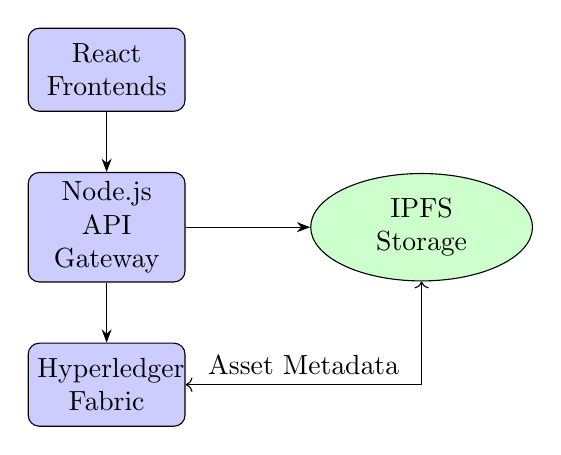
\begin{tikzpicture}[node distance=2cm, auto]
            \tikzstyle{block} = [rectangle, draw, fill=blue!20, text width=5em, text centered, rounded corners, minimum height=3em]
            \tikzstyle{cloud} = [ellipse, draw, fill=green!20, text width=5em, text centered, minimum height=2em]
            
            \node [block] (ui) {React Frontends};
            \node [block, below of=ui] (api) {Node.js API Gateway};
            \node [block, below of=api] (fabric) {Hyperledger Fabric};
            \node [cloud, right of=api, node distance=4cm] (ipfs) {IPFS Storage};
            
            \path [draw, -{Stealth}] (ui) -- (api);
            \path [draw, -{Stealth}] (api) -- (fabric);
            \path [draw, -{Stealth}] (api) -- (ipfs);
            \path [draw, <->] (fabric) -| node [near start] {Asset Metadata} (ipfs);
        \end{tikzpicture}
    \end{center}
    \begin{itemize}
        \item \textbf{Blockchain:} Stores transaction history and data metadata.
        \item \textbf{IPFS:} Stores actual files, with hashes recorded on-chain.
    \end{itemize}
\end{frame}

% Slide 6: System Architecture Overview
\begin{frame}{System-Level Architecture}
    \begin{center}
        \includegraphics[width=0.9\textwidth]{docs/architecture_diagram.png}
    \end{center}
    \vfill
    \begin{itemize}
        \item \textbf{Fabric Network:} 1 Organization, 3 Peers, Raft-based Orderer.
        \item \textbf{Network Mesh:} Tailscale Wireguard for secure communication.
        \item \textbf{Orchestration:} Docker Swarm for high availability.
    \end{itemize}
\end{frame}

% Slide 7: Multi-Node Deployment (Swarm)
\begin{frame}{Distributed Infrastructure}
    MedBlock v2 is deployed across three physical/virtual machines:
    \begin{table}
        \tiny
        \begin{tabular}{|l|l|l|}
            \hline
            \textbf{Node} & \textbf{Role} & \textbf{Components} \\ \hline
            PC1 (Manager) & Swarm Manager & Orderer, CA, Peer0, API, Frontends \\ \hline
            PC2 (Worker) & Swarm Worker & Peer1, CouchDB1 \\ \hline
            PC3 (Worker) & Swarm Worker & Peer2, CouchDB2 \\ \hline
        \end{tabular}
    \end{table}
    \vfill
    \begin{itemize}
        \item \textbf{Inter-node Sync:} Scripts automate synchronization of crypto-artifacts to all worker nodes.
        \item \textbf{Service Discovery:} Swarm handles routing requests to the correct peer container across nodes.
    \end{itemize}
\end{frame}

% Slide 8: Hyperledger Fabric Network Details
\begin{frame}{Hyperledger Fabric Implementation}
    \begin{itemize}
        \item \textbf{Version:} v2.5 (Current LTS).
        \item \textbf{Consensus:} Raft (Ordering Service).
        \item \textbf{MSP:} Org1 managed via Fabric CA.
        \item \textbf{Communication:} Mutual TLS enabled for all peer-to-peer and client-to-peer calls.
    \end{itemize}
    \vfill
    \begin{block}{Network Characteristics}
        All nodes are registered with the Fabric Certificate Authority (CA), ensuring only authorized entities can participate.
    \end{block}
\end{frame}

% Slide 9: Channel and Organization Setup
\begin{frame}{Channel Configuration}
    \begin{itemize}
        \item \textbf{Channel Name:} \texttt{mychannel}
        \item All three peers (Peer0, Peer1, Peer2) are joined to this channel.
        \item \textbf{Anchor Peers:} Peer0 acts as the anchor peer for Org1 to facilitate gossip-based discovery.
        \item \textbf{Channel Policies:} Majority endorsement required for committing transactions.
    \end{itemize}
    \vfill
    \begin{center}
        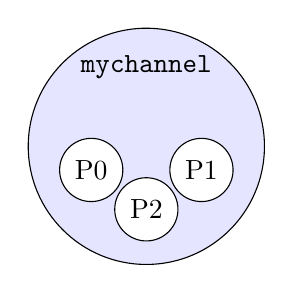
\begin{tikzpicture}
            \draw[fill=blue!10] (0,0) circle (1.5cm);
            \node at (0,1) {\texttt{mychannel}};
            \node[draw, circle, fill=white] at (-0.7, -0.3) {P0};
            \node[draw, circle, fill=white] at (0.7, -0.3) {P1};
            \node[draw, circle, fill=white] at (0, -0.8) {P2};
        \end{tikzpicture}
    \end{center}
\end{frame}

% Slide 10: Smart Contract: EHR Chaincode
\begin{frame}{Chaincode: The Business Logic}
    \begin{itemize}
        \item \textbf{Language:} Node.js (JavaScript).
        \item \textbf{Assets managed:}
        \begin{itemize}
            \item \texttt{PatientRecord}: Demographics, illness history.
            \item \texttt{Prescription}: Medication details, issuance date.
            \item \texttt{AccessGrant}: Permissions for doctors/pharmacists.
        \end{itemize}
        \item \textbf{Queries:} Uses CouchDB selectors for rich attribute-based filtering.
    \end{itemize}
\end{frame}

% Slide 11: Chaincode Functions
\begin{frame}[fragile]{Core Chaincode Functions}
    \begin{lstlisting}[language=JavaScript]
async createPatient(ctx, id, name, dob, gender) {
    const record = { id, name, dob, gender, records: [], docType: 'patient' };
    await ctx.stub.putState(id, Buffer.from(JSON.stringify(record)));
}

async addMedicalRecord(ctx, patientId, diagnosis, ipfsHash) {
    const record = await this.readPatient(ctx, patientId);
    record.records.push({ diagnosis, ipfsHash, timestamp: new Date() });
    await ctx.stub.putState(patientId, Buffer.from(JSON.stringify(record)));
}
    \end{lstlisting}
    \vfill
    \textit{Note: All functions require valid identity certificates for execution.}
\end{frame}

% Slide 12: IPFS Storage Integration
\begin{frame}{Off-Chain Storage: IPFS}
    \textbf{Why IPFS?}
    Blockchain is expensive for large data. We store heavy files on IPFS and keep the hash on the Ledger.
    \vfill
    \begin{center}
        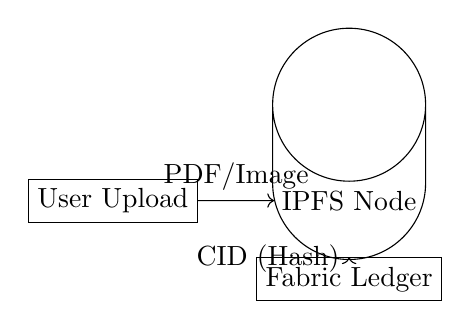
\begin{tikzpicture}[auto]
            \node[draw, rectangle] (local) {User Upload};
            \node[draw, cylinder, right of=local, node distance=3cm, shape border rotate=90] (ipfs) {IPFS Node};
            \node[draw, rectangle, below of=ipfs] (ledger) {Fabric Ledger};
            
            \path [draw, ->] (local) -- node {PDF/Image} (ipfs);
            \path [draw, ->] (ipfs) -- node {CID (Hash)} (ledger);
        \end{tikzpicture}
    \end{center}
    \begin{itemize}
        \item \textbf{Content Addressing:} Files are immutable because changing a file changes the Hash.
        \item \textbf{Process:} Frontend $\to$ Backend API $\to$ IPFS $\to$ Fabric Ledger.
    \end{itemize}
\end{frame}

% Slide 13: Frontend: Manager Dashboard
\begin{frame}{Manager Portal: Governance}
    \begin{columns}
        \begin{column}{0.5\textwidth}
            \begin{itemize}
                \item \textbf{User Management:} Register new Doctors, Pharmacists, and Patients.
                \item \textbf{Network Stats:} Monitor Fabric Peer health and Swarm status.
                \item \textbf{Auditing:} View system-wide logs of credential issuance.
            \end{itemize}
        \end{column}
        \begin{column}{0.5\textwidth}
            \begin{center}
                \textit{(Placeholder for Manager UI Screenshot)}
                \draw[thick] (0,0) rectangle (3,2);
                \node at (1.5, 1) {\tiny GLASSMORPHIC UI};
            \end{center}
        \end{column}
    \end{columns}
\end{frame}

% Slide 14: Frontend: Pharmacist \& Billing
\begin{frame}{Pharmacist \& Billing Portal}
    \begin{itemize}
        \item \textbf{Prescription Lookup:} Securely read prescriptions authorized for the patient.
        \item \textbf{Billing Integration:} Automatically calculate costs based on prescribed medicine.
        \item \textbf{Ledger Record:} Every bill payment recorded as a transaction on Fabric.
    \end{itemize}
    \vfill
    \begin{block}{Key Feature}
        Pharmacists can only view relevant medication data, protecting patient's primary diagnosis privacy.
    \end{block}
\end{frame}

% Slide 15: Frontend: Inventory Management
\begin{frame}{Inventory Management Dashboard}
    \begin{itemize}
        \item \textbf{Stock Tracking:} Real-time updates on medicine availability.
        \item \textbf{Supply Chain Trust:} Verify the batches medicine from suppliers (Future Scope).
        \item \textbf{Integration:} Linked with the Billing portal to decrement stock on purchase.
    \end{itemize}
    \vfill
    \begin{center}
        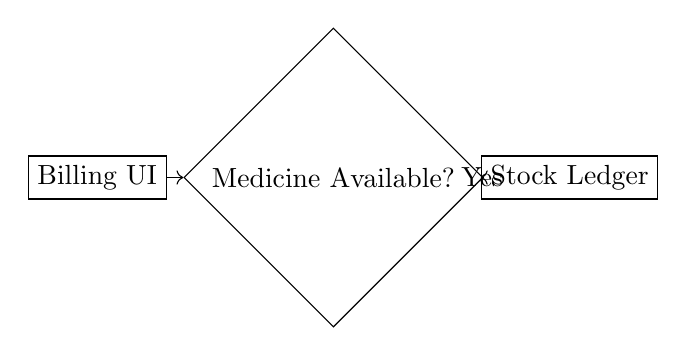
\begin{tikzpicture}
            \node[draw, diamond] (stock) {Medicine Available?};
            \node[draw, rectangle, left of=stock, node distance=3cm] (billing) {Billing UI};
            \node[draw, rectangle, right of=stock, node distance=3cm] (ledger) {Stock Ledger};
            \path [draw, ->] (billing) -- (stock);
            \path [draw, ->] (stock) -- node {Yes} (ledger);
        \end{tikzpicture}
    \end{center}
\end{frame}

% Slide 16: Frontend: Patient Health Records
\begin{frame}{Patient Self-Governance Portal}
    Empowering patients with their own medical data.
    \vfill
    \begin{itemize}
        \item \textbf{Personal History:} View complete chronological medical history.
        \item \textbf{Report Access:} Download medical reports (via IPFS).
        \item \textbf{Identity Management:} Secure login using Fabric Wallet certificates.
        \item \textbf{Privacy Control:} Patients are the owners of their identity (Self-Sovereign Identity concepts).
    \end{itemize}
\end{frame}

% Slide 17: Backend API Architecture
\begin{frame}{Backend: The Bridge}
    \begin{itemize}
        \item \textbf{Technology:} Express.js / Node.js.
        \item \textbf{Fabric SDK:} Uses \texttt{fabric-network} library to connect to gateways.
        \item \textbf{Wallet Management:} Stores FileSystemWaypoints for user private keys (\texttt{.id} files).
        \item \textbf{Concurrency:} Handles multiple simultaneous transaction requests from disparate frontends.
    \end{itemize}
\end{frame}

% Slide 18: Security \& Identity Management
\begin{frame}{Security Infrastructure}
    \begin{itemize}
        \item \textbf{PKI (Public Key Infrastructure):} Every user has an X.509 certificate.
        \item \textbf{Attribute Based Access Control (ABAC):} User roles (Manager, Patient, etc.) are embedded in the certificate.
        \item \textbf{Mutual TLS:} Encrypted communication channels between nodes.
        \item \textbf{Data Security:} Hashes prevent data tampering; IPFS ensures data persistence.
    \end{itemize}
\end{frame}

% Slide 19: Deployment Automation
\begin{frame}[fragile]{One-Click Deployment}
    Automated deployment via \texttt{deploy.sh}:
    \begin{itemize}
        \item \textbf{Step 1:} Initialize Swarm Network on PC1.
        \item \textbf{Step 2:} Generate Crypto-materials on PC1.
        \item \textbf{Step 3:} Sync artifacts (configs, IDs) to Worker Nodes via SCP.
        \item \textbf{Step 4:} Spin up Fabric CA, Orderers, and Peers.
        \item \textbf{Step 5:} Deploy React Apps and Node.js API.
    \end{itemize}
\end{frame}

% Slide 20: Conclusion \& Future Work
\begin{frame}{Conclusion}
    \begin{itemize}
        \item \textbf{Summary:} Successfully implemented a decentralized, multi-node EHR platform.
        \item \textbf{Impact:} Enhanced data security, trust between medical entities, and patient empowerment.
    \end{itemize}
    \vfill
    \textbf{Future Work:}
    \begin{itemize}
        \item AI-based diagnosis assistance.
        \item Multi-organization (Cross-Hospital) network expansion.
        \item Integration with IoT-based health monitoring devices.
    \end{itemize}
\end{frame}

% Final Slide
\begin{frame}
    \begin{center}
        \Huge \textbf{Thank You!} \\
        \vfill
        \Large Questions? \\
        \vfill
        \small Team: Ankit, Mohit, Ronit
    \end{center}
\end{frame}

\end{document}
